% ============================================================
\section{Introduction}
\label{sec:intro}
Suppose the Federal Reserve leaves the policy rate unchanged. In one month stock prices fall; in another the dollar appreciates. Both movements tend to restrain spending. How much tightening has each delivered? One way to answer is to ask how large a monetary policy surprise would ordinarily produce a comparable movement in financial markets. Another is to ask how large a change in the policy rate would have a comparable effect on spending. A policymaker might reasonably expect the two answers to be close.

The two questions are different, and the difference is real. It does not, however, settle the answer. Figure~\ref{fig:four} applies four calibrations to the same two movements: a 5 log point fall in equity valuation and a 3.9 log point appreciation of the dollar, with the 10-year yield unchanged. I chose the sizes so that the market index built from the futures-based measure of policy news rates the two alike. Two calibrations read the dollar movement as about as tight as the equity movement: that market index (a ratio of \bl{fw:fig:F}) and the published Goldman Sachs weights, which are calibrated to effects on GDP (\bl{fw:fig:G}). Two read it as more than twice as tight: the market index built from the change in the two-year yield (\bl{fw:fig:Y}) and the Federal Reserve's FRB/US model (\bl{fw:fig:B}). The split runs across the two methods, not between them.

\begin{figure}[tbp]
\centering
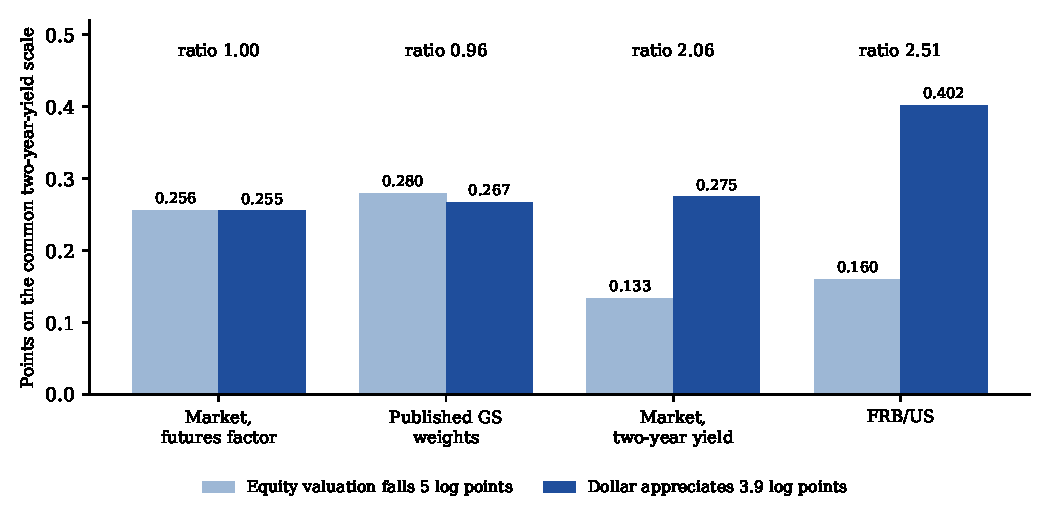
\includegraphics[width=0.9\textwidth]{../replication/report/fig_four.pdf}
\caption{Two Tightenings Read by Four Calibrations}
\label{fig:four}
\begin{flushleft}\footnotesize\textit{Notes:} Readings of each movement under four portfolios of the same three assets relative to $r^*$, each normalized to read one on the response of the three assets to one unit of policy news measured by the futures factor (points on the common two-year-yield scale). Market: weights from announcement-window responses, with policy news measured by the futures factor or by the change in the two-year yield. FRB/US: effects on GDP after four quarters of persistent shifts. Published GS weights: the U.S.\ weights on the 10-year yield, equities and the dollar reported by \citet{caballero2026b}, applied to the series used here with the GS policy-rate and spread terms held fixed. The ratio above each pair is the dollar reading over the equity reading; it does not depend on the normalization. The sizes of the movements were chosen to give equal readings under the futures factor; the ratio of one calibration's ratio to another's does not depend on that choice.\end{flushleft}
\end{figure}

\citet{caballero2026b} give a related example with the published Goldman Sachs weights: a 20 percent fall in U.S.\ equity prices and a 17 percent appreciation of the currency each tighten the index by about one point, because equities carry a small weight and move a lot, and the exchange rate carries a larger weight through expenditure switching. Applied to the movements of Figure~\ref{fig:four}, the same weights give a ratio of \bl{fw:gsraw}.

The choice matters for real decisions. In 2008--09, when equity valuations collapsed, all four calibrations registered a large tightening over the year, but the futures-factor and GS readings averaged \bl{fw:ep:200809:F} and \bl{fw:ep:200809:G} points and the two-year-yield and FRB/US readings \bl{fw:ep:200809:Y} and \bl{fw:ep:200809:B}. The direction was clear; the size differed by more than half a point, an amount worth discussing at a policy meeting.

Policymakers read the stance of policy from financial conditions. In November 2023 the Chair noted that ``Financial conditions have tightened significantly in recent months, driven by higher longer-term bond yields, among other factors'' \citep{powell2023}, and in March 2024 that ``there are many different financial conditions indicators, and you can kind of, you know, see different answers to that question'' \citep{powell2024}. A reading of financial conditions is a reading of policy only to the extent that a point of the index means a point of policy. This paper asks how many points of policy a movement in financial conditions is worth under four calibrations, whether knowing how an index was built predicts its reading, whether the choice would have changed the reading of history, and whether later activity favors any calibration.

I find that knowing how an index was constructed tells a reader surprisingly little about which other index it will resemble. I put the four calibrations on one scale, on which each reads one on the futures-factor response to policy news, and apply them to every 12-month change in the three assets from 1996 to 2026. Across the four calibrations, financial conditions usually give the same directional signal. All four readings have the same sign in \bl{fw:all:same:sign} percent of the \bl{fw:nmonths} months, and at least two give materially opposing readings, each at least 25 basis points from zero, in \bl{fw:any:opposing:t25:n} months. The size of the tightening is more sensitive. Switching between the two market calibrations moves the reading by \bl{fw:mad:FY} basis points on average, and switching between FRB/US and the published Goldman Sachs weights by \bl{fw:mad:BG}, against \bl{fw:mad:FB} for the futures-factor market index and FRB/US. Switching between two implementations of the same method can change the reading as much as switching from market responses to spending effects. The two closest readings in the sample come from different methods: the futures-factor market index and the published Goldman Sachs weights differ by \bl{fw:mad:FG} basis points on average. That is a ranking of point estimates; the distances have wide intervals. The ranking does not come from the transformations of the series: on the real 10-year yield, the log of the cyclically adjusted price-earnings ratio and the real dollar, and on the nominal 10-year yield, the same equity measure and the nominal dollar, the futures-factor and GS readings remain the closest pair, and a within-method distance remains at least as large as the featured cross-method distance.

The paper also explains why the weights differ. On the same announcements, the part of the two-year yield change that the futures factor does not capture moves long yields and the dollar and not equities, so a market index built to recover the two-year yield puts less weight on equities. In FRB/US, net exports carry almost all of the effect of the dollar on GDP, and consumption most of the effect of equities. Why the published Goldman Sachs weights line up with the futures-factor market weights is a finding whose cause the paper leaves open.

The exceptions to directional agreement are concentrated. At 25 basis points, adding the other two calibrations produces no month of material opposition beyond the \bl{fw:fb25:n} of the futures-factor and FRB/US pair; at 10 basis points it doubles the count, from \bl{fw:fb10:n} to \bl{fw:any:opposing:t10:n}. In \bl{fw:opp25:Balone} of the \bl{fw:any:opposing:t25:n} months of materially opposing readings, FRB/US alone reads a tightening that the others read as an easing, in late 1997 and 1998 and in early 2015, when the dollar and valuations had both risen by more than 10 percent over the year. In the other \bl{fw:opp25:FGtight}, in 2003 and 2008, the futures-factor and Goldman Sachs readings were tight and FRB/US was easy. The four readings are furthest apart in 2008 and 2009, and in 2022--24 every calibration shows a tightening of about one point or more. Aggregate unemployment and GDP growth do not separate the calibrations, and the tests have little power.

The paper has five further parts. Section~\ref{sec:indexes} defines a policy equivalent under each method. Section~\ref{sec:agree} explains why the weights differ: the measure of policy news on the market side, the expenditure channels and the published weights on the spending side, and the role of persistence in the conversion. Section~\ref{sec:history} puts the four calibrations on one scale, reads three episodes with them and asks how often the choice changes the judgment over the full history. Section~\ref{sec:outlook} asks what subsequent activity can establish, and Section~\ref{sec:limitsmain} examines the stability of the weights and the limits of the design.

\subsection{Connection to the Literature}
\textbf{Weights and their meaning.} Indexes of financial conditions differ mainly in the source of their weights \citep{hatzius2010}: effects on output from a model \citep{dudley2000,hatzius2018,ajello2023}, principal components \citep{brave2011}, or event-study regressions \citep{kuttner2001,gurkaynak2005,bernanke2005,nakamura2018,bauer2023}. The older literature on monetary conditions indexes recognized that the weights on asset prices depend on the shock and the dynamics, so that their policy meaning is not invariant \citep{eika1996}. I quantify that difficulty with four sets of U.S.\ weights on common assets and ask where it matters.

\textbf{The closest comparisons.} \citet{arnaut2024} estimate how an existing index responds to policy surprises, \citet{sack2023} relate FCI-G to policy-induced changes in the two-year yield, and \citet{ajello2023} translate movements into a growth impulse with model multipliers. \citet{bletzinger2026} build a U.S.\ macro-finance index in units comparable to a policy rate and compare it with the Goldman Sachs index and FCI-G, finding divergences driven by equities and the strongest tightening in 2022--24. Comparisons of published indexes mix the weights with differences in assets, transformations and units. My design holds the assets, the transformations and the policy unit fixed across calibrations, so that a difference in readings can be attributed to the weights. \citet{boehm2025} show that announcements also move equities and exchange rates along a dimension orthogonal to yield changes, so a movement that departs from the conventional pattern can come from the announcement itself.

\textbf{Information about activity.} \citet{hatzius2010} build an index conditional on past activity and inflation, \citet{aramonte2013} show that comparisons among indexes depend on the crisis in the sample, and \citet{lombardi2025} separate safe yields from priced risk and find that risk predicts activity more strongly. \citet{adrian2019} show that conditions shift the lower quantiles of growth, and \citet{brave2011} build an index of risk, credit and leverage. \citet{caballero2026} define FCI$^*$, the level of financial conditions consistent with output at potential. The neutral rate matters for the level of every index \citep{laubach2003,holston2017,holston2023,hamilton2016,bauer2020,kiley2020}; I measure the inputs relative to $\rs$ and do not estimate a neutral level for the index (Appendix~\ref{app:steps}).
\textbf{Why the meaning of a point matters.} \citet{caballero2024} study targeting an index of financial conditions in a closed economy, and \citet{caballero2026b} extend the analysis to a multi-asset open economy, in which domestic asset prices and the exchange rate both enter aggregate demand and policy responses link the markets. That gives a reason to care which mix of asset prices delivers a given index reading. My question comes one step earlier: when does a portfolio inferred from conventional policy news give those markets the same relative importance as a spending calibration? The answer does not require endorsing targeting. The same ambiguity arises for anyone who communicates about a desired path of financial conditions, since the path has to say what a point on it means, and for a neutral benchmark such as FCI$^*$ \citep{caballero2026}, which takes the aggregation of asset movements as given.
\FloatBarrier

% ============================================================
\section{Two Ways to Read a Financial Movement}\label{sec:indexes}
\subsection{Two Meanings of a Policy Equivalent}\label{sec:meanings}
Take a movement in three asset prices: the 10-year Treasury yield, equity valuation and the real broad dollar. Each is measured relative to $r^*$ and to its 1973--2026 average (Appendix~\ref{app:steps}). I call a reading of the movement a policy equivalent if it says how much tightening of the policy rate the movement amounts to. There are two natural ways to compute one.

The market index starts from policy. At each Federal Open Market Committee announcement I measure the policy surprise with the factor of \citet{nakamura2018}, scaled so that one unit raises the two-year yield by one percentage point, and I measure how the three asset prices respond in a narrow window around the announcement. The weights are chosen to recover the size of the surprise from the three asset prices together. A movement is then worth the size of the surprise that would, on average, produce it, in points of the two-year yield. A policy surprise of one unit reads one. I call this the market-implied reading.

The FRB/US index starts from spending. Each asset price is weighted by its effect on GDP four quarters later in the Federal Reserve's FRB/US model \citep{brayton2014}, in the experiment in which the asset price shifts persistently, divided by the effect of a persistent one percentage point rise in the federal funds rate. A movement is then worth the funds-rate change with the same effect on GDP, in funds-rate points. I call this the spending-equivalent reading.

The first calculation reads a movement through what policy does to markets. The second reads it through what markets do to spending. Both are legitimate. They need not agree.

\subsection{Why the Weights Differ}\label{sec:why}
Consider the dollar. It can be a reliable indicator of a policy surprise because it responds consistently when the expected path of U.S.\ interest rates changes. How useful it is as an indicator depends on how much it also moves for other reasons, and on what yields and equities already reveal. Its weight in a spending index depends on different things: how an appreciation affects net exports, and how long the appreciation lasts. An asset can be an excellent indicator of a policy surprise and have a modest effect on spending. It can also be a noisy indicator and have a large effect on spending. The same is true of equities, whose effect on spending runs through wealth and the cost of capital. A fall in equity prices that reflects a higher discount rate is policy-like, and a fall that reflects weaker earnings prospects is not policy at all. The event study averages over announcements, where the first kind dominates. The model prices an equity movement by its estimated effect on spending, whatever its source. Neither calculation is wrong about its own question.

Two equations make the argument precise. Let $x$ be the movement in the three asset prices around an announcement, $s$ the policy surprise, and $\psi$ the vector of responses of the asset prices to a unit of surprise:
\begin{equation}\label{eq:decomp}
x=\psi s+u .
\end{equation}
The vector $u$ collects the ways in which a particular movement departs from the usual response to conventional rate news. It has covariance $\Sigma$. Even an announcement can produce such a departure. The market weights $w_M$ recover $s$ from $x$ by generalized least squares, $w_M\propto\Sigma^{-1}\psi$, normalized so that $w_M'\psi=1$. The FRB/US weights $b_h$ are the effects of the three asset prices on GDP at horizon $h$ in funds-rate points. The model prices the usual response $\psi$ at $b_h'\psi$, which I report in its own units, and dividing by it gives the normalized weights $w_{B,h}=b_h/(b_h'\psi)$, so that both indexes read one on a conventional policy surprise. The difference between the two readings of a movement $x$ is then
\begin{equation}\label{eq:D}
D_h(x)=(w_{B,h}-w_M)'x=(w_{B,h}-w_M)'u ,
\end{equation}
because the policy part $\psi s$ cancels. The same difference has a second reading. The fitted policy component of any movement $x$ is $\psi M$, where $M=w_M'x$ is the market-implied reading; the remainder $x-\psi M$ is the combination of asset prices that a conventional policy surprise cannot reproduce. Once the scales are matched, the spending-equivalent valuation of that remainder is precisely the difference between the two readings,
\begin{equation}\label{eq:rem}
D_h(x)=w_{B,h}'(x-\psi M),
\end{equation}
because $w_{B,h}'\psi=1$. A reader can say what the difference measures without assigning it a structural cause. The argument extends to any two portfolios normalized to read one on the usual policy response: their difference prices only the part of an observed movement outside that response. That is the bridge from two methods to four calibrations. It also means that an arbitrary movement can read as one point of tightening under every calibration, and so resemble a policy tightening, even when no policy shock produced it. In words, the two methods disagree only to the extent that asset prices move in unusual proportions and the methods value those departures differently. An unusual movement is not enough by itself: if the weights are the same, there is nothing to value differently. A difference in weights is not enough either: if the asset prices keep moving together as they do around policy news, the difference has nothing to act on. That is why two indexes can track each other closely for decades and still give different readings during an equity boom or a dollar surge. Throughout, $D$ is the difference computed on the movements of the three asset prices over the horizon in question, and in Section~\ref{sec:outlook} it is computed on 12-month changes. Appendix~\ref{app:ma} derives the weights.

\subsection{Putting Numbers on It}\label{sec:requires}
Figure~\ref{fig:four} applies four sets of weights to two movements. Neither movement is a policy surprise, so nothing in the construction requires the readings to agree. For an equity decline of size $e$ and a dollar appreciation of size $d$, the ratio of one calibration's dollar-to-equity reading to another's does not depend on $e$ or $d$, because $d/e$ cancels; the choice of movements fixes the futures-factor ratio at one and sets the gap in basis points, not the relative weights. Table~\ref{tab:example} gives the FRB/US readings in its own units, funds-rate points, before any normalization. Whether the differences are large in practice depends on how often asset prices move in such proportions, which Sections~\ref{sec:size} and~\ref{sec:history} measure.
\FloatBarrier

% ============================================================
\section{Where the Weights Come From}\label{sec:agree}
Table~\ref{tab:fourw} puts the four sets of weights side by side on the common scale, on which each reads one on the response of the three assets to one unit of futures-factor policy news. The futures-factor market weights and the published GS weights are close on all three assets. The two-year-yield market weights put more weight on the 10-year yield and half as much on equities. FRB/US puts the most weight on the dollar relative to equities. This section explains the two differences the paper can trace: why a different measure of policy news lowers the market equity weight, and why the dollar matters for GDP in FRB/US.

\begin{table}[tbp]\centering
\caption{Four Sets of Weights on One Scale}\label{tab:fourw}
\resizebox{\ifdim\width>\textwidth\textwidth\else\width\fi}{!}{%
\begin{tabular}{lcccc}
\toprule
 & Market, futures factor & Published GS weights & Market, two-year yield & FRB/US \\
\midrule
10-year yield (per percentage point) & 0.609 [0.147, 1.114] & 0.515 & 0.926 [0.476, 1.328] & 0.590 \\
Equity valuation (per log point) & $-$0.051 [$-$0.068, $-$0.030] & $-$0.056 & $-$0.027 [$-$0.046, $-$0.011] & $-$0.032 \\
Dollar (per log point) & 0.065 [0.021, 0.112] & 0.069 & 0.070 [0.033, 0.110] & 0.103 \\
\bottomrule
\end{tabular}}
\begin{flushleft}\footnotesize\textit{Notes:} Weights on the three assets relative to $r^*$, each set normalized to read one on the response of the three assets to one unit of futures-factor policy news (the common two-year-yield scale). Market weights: generalized least squares on 253 announcement windows, with policy news measured by the futures factor or by the change in the two-year yield; brackets are 90 percent intervals over 5,000 bootstrap draws of the announcements (for the two-year-yield weights, of the weights on their own signal, which differ from the entries by a factor of \bl{fw:wYpsiF}). FRB/US: effects on GDP after four quarters of persistent shifts. Published GS weights: the U.S.\ weights on the 10-year yield, equities and the dollar, with the GS policy-rate and spread terms held fixed. The FRB/US and GS weights are not estimated here.\end{flushleft}
\end{table}


\subsection{One Set of Announcements, Two Measures of Policy News}\label{sec:signal}
The market weights come from the \bl{n:events} announcements from \bl{event:first} to \bl{event:last} in the San Francisco Fed's U.S.\ Monetary Policy Event-Study Database \citep{acosta2025}. In a narrow window around each announcement I measure the responses of the 10-year yield, the S\&P 500 and the dollar. The weights recover a specified measure of the policy news from the three responses together, so the definition of policy news is a measurement choice. Two measures are natural on these announcements. The baseline is the futures-based factor of \citet{nakamura2018}. The alternative is the change in the two-year Treasury yield in the same windows, which is the unit in which the market index is quoted.

The two measures share most of their variation. Their correlation is \bl{sig:corr}. Write the two-year change as the factor plus a remainder. The remainder is \bl{sp:resvar} percent of the variance of the two-year change (interval \bl{sp:resvar:lo} to \bl{sp:resvar:hi} percent), about \bl{sp:ressd} percent of its standard deviation. Figure~\ref{fig:signal} shows which assets move with each part. A point of the factor raises the 10-year yield by \bl{sp:ten:F} points, lowers the S\&P 500 by \bl{abs:sp:eq:F} percent and raises the dollar by \bl{sp:usd:F} percent. A point of the remainder is associated with a rise in the 10-year yield of \bl{sp:ten:R} points and in the dollar of \bl{sp:usd:R} percent, and with an equity response of \bl{sp:eq:R} percent (\bl{sp:eq:R:lo} to \bl{sp:eq:R:hi}) that the data cannot distinguish from zero.

\begin{figure}[tbp]
\centering
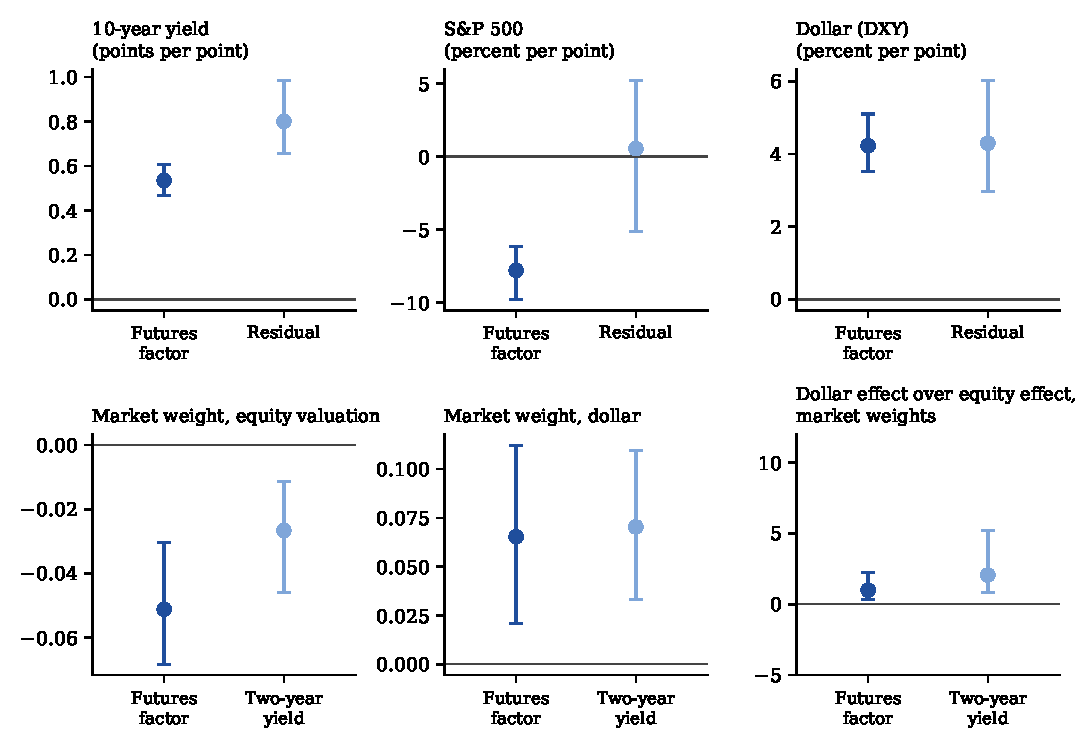
\includegraphics[width=\textwidth]{../replication/report/fig_signal.pdf}
\caption{What the Two Measures of Policy News Capture}
\label{fig:signal}
\begin{flushleft}\footnotesize\textit{Notes:} Top: responses of the 10-year yield (points), the S\&P 500 and the dollar (DXY) (percent) in the announcement windows to one point of the futures factor and to one point of the part of the two-year yield change that is orthogonal to it; the factor is scaled to the two-year change. Bottom: the market weight on equity valuation and on the dollar, and the market's dollar-over-equity effect ratio, when policy news is measured by the futures factor and by the two-year yield. Bars are 90 percent intervals from 5,000 bootstrap draws of the announcements, drawn in common for the two signals.\end{flushleft}
\end{figure}

Table~\ref{tab:weights} gives the market weights under the baseline. A policy move that raises the two-year yield by one point raises the 10-year yield by \bl{psi:ten} points, lowers equity valuation by \bl{abs:psi:eq} percent and raises the real dollar by \bl{psi:usd} percent. Each variable carries a substantial part of the policy move, with shares of \bl{share:ten} for the 10-year yield, \bl{share:eq} for equity valuation and \bl{share:usd} for the dollar.

\begin{table}[tbp]\centering\small
\caption{Market Index: Responses to Policy News and Weights}\label{tab:weights}
\resizebox{\ifdim\width>\textwidth\textwidth\else\width\fi}{!}{%
\begin{tabular}{lrrrr}
\toprule
 & Response & Weight & 90\% interval & Share of policy move \\
\midrule
10-year Treasury yield (pp) & 0.53 (0.06) & 0.609 & [0.147, 1.114] & 0.33 \\
Equity valuation, 100 ln CAPE (percent) & $-$7.78 (0.93) & $-$0.051 & [$-$0.068, $-$0.030] & 0.40 \\
Real broad dollar, 100 ln (percent) & 4.22 (0.53) & 0.065 & [0.021, 0.112] & 0.28 \\
\bottomrule
\end{tabular}}
\begin{flushleft}\footnotesize\textit{Notes:} Announcement windows, 253 announcements, January 1996 to September 2026. Response: change in the window per unit of policy news, which moves the two-year yield by 1 percentage point (heteroskedasticity-robust standard errors in parentheses). Weight: one-factor generalized least squares, normalized so that the weights applied to the responses sum to 1. Interval: 5th and 95th percentiles of weights re-estimated on 5000 bootstrap samples of the announcements. Share: weight times response.\end{flushleft}
\end{table}


\textbf{Why the equity weight falls.} The weights are the generalized least squares weights that recover the signal, $w_M\propto\Sigma^{-1}\psi$. When the signal is the two-year yield, the remainder becomes part of the signal and not part of the noise. Because the remainder moves yields and the dollar and not equities, equity valuation responds less per unit of the signal and is a weaker indicator of it. The equity weight falls from \bl{sg:base:weq} to \bl{sg:two:weq}. Switching the response vector and the residual covariance in turn, each accounts for about half of the change (\bl{sig:cf:psi} and \bl{sig:cf:sig}), and the order does not matter. The market's dollar-to-equity weight ratio under the two-year yield is \bl{tp:two:rr} times its ratio under the factor, with a paired 90 percent interval of \bl{tp:two:rr:lo} to \bl{tp:two:rr:hi}. I report the roughly twofold change as a point estimate. The regressions show what variation each measure captures. They do not show whether the remainder is further policy news, a term-premium movement or measurement error.

\textbf{What the weights say.} The weights say what the variables do when policy moves, not what causes their movements at other times. A rise in stock prices that comes from news about earnings has little to do with policy, and the index treats it as if it did. An announcement can also reveal the Fed's view of the economy, and then the responses mix policy and information \citep{nakamura2018}. I measure the responses as markets receive them and set the information effect aside. The index measures policy-equivalent tightening. It is not a forecast of activity.

\textbf{Readings of the two movements.} Table~\ref{tab:signal} in the appendix applies the weights, normalized for each signal, to the movements of Figure~\ref{fig:four}. The market-implied reading rates the equity decline and the dollar appreciation \bl{sg:base:cm} apart with the futures factor and \bl{sg:two:cm} apart with the two-year yield. The model rates the dollar movement \bl{sg:base:cf} points tighter than the equity movement. The model less market contrast is \bl{sg:base:contrast:diff} (90 percent interval \bl{sg:base:contrast:diff:lo} to \bl{sg:base:contrast:diff:hi}) for the baseline and \bl{sg:two:contrast:diff} (\bl{sg:two:contrast:diff:lo} to \bl{sg:two:contrast:diff:hi}) for the two-year yield. On common draws, switching from the futures factor to the two-year yield lowers the contrast by \bl{pr:two:contrast:bp} basis points of the two-year yield (\bl{pr:two:contrast:diff:d}, interval \bl{pr:two:contrast:diff:dlo} to \bl{pr:two:contrast:diff:dhi}). The model gives the dollar more weight relative to equities than the market does in the point estimates under both measures, and the interval for the difference includes zero under the two-year yield.


\textbf{Proportionality.} Whether the model's dollar-to-equity weight ratio equals the market's is a question about relative weights and not about size. The cross-product $c=w_{B,\$}w_{M,E}-w_{B,E}w_{M,\$}$ is zero if and only if they are equal. Its 90 percent interval excludes zero for the futures factor (\bl{pr:base:cross}, \bl{pr:base:cross:lo} to \bl{pr:base:cross:hi}) and includes it for the two-year yield (\bl{pr:two:cross}, \bl{pr:two:cross:lo} to \bl{pr:two:cross:hi}). The ratio of the model's ratio to the market's, which is \bl{sg:base:ror} for the baseline and \bl{sg:two:ror} for the two-year yield (interval \bl{sg:two:ror:lo} to \bl{sg:two:ror:hi}), tests the same hypothesis on a scale-free ratio, but its denominator, the market's equity effect, is small and imprecise. The two sample checks, announcements through 2019 and outside the lower-bound years, give contrasts of \bl{sg:t19:contrast:diff} (\bl{sg:t19:contrast:diff:lo} to \bl{sg:t19:contrast:diff:hi}) and \bl{sg:nlb:contrast:diff} (\bl{sg:nlb:contrast:diff:lo} to \bl{sg:nlb:contrast:diff:hi}); Appendix~\ref{sec:robother} reports them. The intervals are not adjusted for the number of definitions.

\subsection{How Precisely Are the Weights Estimated?}\label{sec:precision}
The weights come from regressions on \bl{n:events} announcements. The weight on the 10-year yield has a 90 percent interval from \bl{wb:ten:lo} to \bl{wb:ten:hi} around \bl{w:ten}. The interval for equity valuation runs from \bl{wb:eq:lo} to \bl{wb:eq:hi}, and for the dollar from \bl{wb:usd:lo} to \bl{wb:usd:hi}. The FRB/US weights on all three lie inside these intervals, the equity weight near the edge: it is lower in absolute value than \bl{frw:eq:pct} percent of the bootstrap draws, about 14 percent in a two-sided test. The data do not reject that the model weights equal the market weights. This is a statement about power, not a finding that they are equal, and it treats the FRB/US weights as fixed. The intervals in the text come from the bootstrap of the announcements; the contrast in composition in Section~\ref{sec:persist} is the ratio of ratios, whose interval includes one at two quarters.


The intervals behind Figure~\ref{fig:four} and the FRB/US readings in funds-rate points are in Table~\ref{tab:example} in the appendix.


\subsection{Where the Model's Weights Come From}\label{sec:channels}
Table~\ref{tab:frbus} compares the market weights with the FRB/US weights. The two sets agree on the 10-year yield, where the FRB/US weight is \bl{ratio:ten} times the market weight. The model puts less weight on equity valuation (\bl{ratio:eq} times) and more on the dollar (\bl{ratio:usd} times). On a policy move the difference does not matter, because the policy part cancels in equation~(\ref{eq:D}). On a departure from the usual response, the model gives a fall in equity prices its estimated effect on output, and the market index treats it as policy-equivalent.


The FRB/US weights are effects on GDP, and a reader should see where they come from. Figure~\ref{fig:channels} follows the two movements of Figure~\ref{fig:four} through the model under one persistence assumption, a persistent shift. Only the stated variable moves. The policy rate, the Treasury curve, the mortgage and car-loan rates, the BBB spread, equity valuation, household stock wealth and the dollar are held at baseline in every experiment except their own, so the policy rule is inactive and expectations are those of the model's VAR. The GDP object is the percent deviation of real GDP from baseline. The contributions are the model's own expenditure identities, weighted by shares in GDP, and they sum to GDP.

\begin{figure}[tbp]
\centering
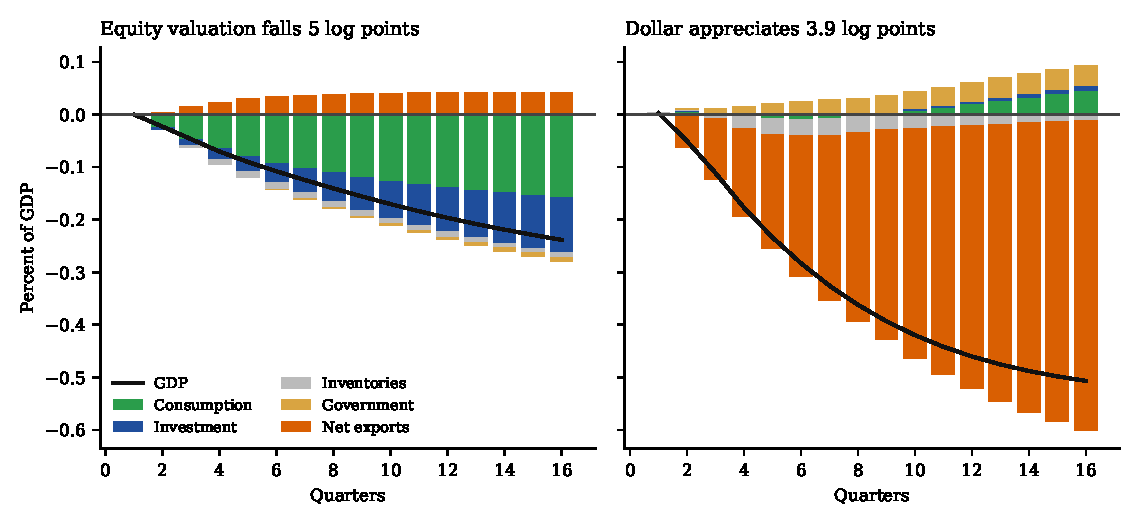
\includegraphics[width=\textwidth]{../replication/report/fig_channels.pdf}
\caption{How the Two Movements Reach GDP in FRB/US}
\label{fig:channels}
\begin{flushleft}\footnotesize\textit{Notes:} Percent deviation of real GDP from baseline and contributions by expenditure component, persistent shift in the variable, other financial variables held at baseline, policy rule inactive. Investment is residential and business fixed investment; net exports are exports less imports. The figure uses the Board's FRB/US package with the data vintage of October 2026, the vintage behind every FRB/US number in the paper.\end{flushleft}
\end{figure}

The equity movement reduces GDP by \bl{ch:gdp:eq} percent after four quarters, and domestic demand accounts for it. Consumption supplies \bl{ch:eq:cons} percent of the effect, through wealth and the cost of capital, and business fixed investment \bl{ch:eq:bfi} percent. Domestic demand in all supplies \bl{ch:eq:dom} percent, and net exports offset \bl{abs:ch:eq:nx} percent of it, because weaker demand reduces imports; inventories supply \bl{ch:eq:inv} percent and government \bl{ch:eq:gov} percent, so that the shares sum to 100. The dollar movement reduces GDP by \bl{ch:gdp:usd} percent, and net exports account for \bl{ch:usd:nx} percent of it: exports \bl{ch:usd:exp} percent and imports \bl{ch:usd:imp} percent. Domestic demand contributes \bl{ch:usd:dom} percent, inventories \bl{ch:usd:inv} percent and government \bl{ch:usd:gov} percent of the GDP effect. With a half-life of four quarters the shares are similar (consumption \bl{ch:eq:cons4} percent of the equity effect and net exports \bl{ch:usd:nx4} percent of the dollar effect). The two weights therefore reflect two different channels, and the dollar's larger weight is a statement about trade. It carries no implication about how persistent the dollar is, which is the assumption of the experiment.

The experiments need two mappings from the market series to the model. The equity experiment shocks the required return on equity, and household stock wealth falls with it in the same simulation, so valuation and wealth move jointly; the 5 log point fall in valuation is entered as a 5 percent fall in stock wealth on impact. The market side measures equity by the S\&P 500 return in the announcement window, which gives the weight on equity valuation, and applies that weight to monthly changes in the earnings-yield gap converted to CAPE log points (Appendix~\ref{app:steps}); a one percent window return is treated as one log point of valuation, with earnings unchanged. The dollar experiment raises the model's real exchange rate by one percent per unit, and the market side measures the dollar by the DXY in the window and applies the weight to the log of the broad real dollar. DXY is a nominal index of six currencies and the model's dollar is a trade-weighted real index. I treat them as the same unit, and over a window or a month the nominal moves dominate.

The model's own policy shock gives a funds-rate equivalent of \bl{ps:ffr} for the usual announcement mix against \bl{ps:replay} for the announcement response. FRB/US can therefore assign a value near one to the observed announcement mix even though its own policy shock generates a different mix: heavier in equities and lighter in the dollar. The comparison is not a decomposition of how much of transmission the three assets omit, because the policy shock changes the path, the equity response, the channels that operate and the unit of normalization together. Appendix~\ref{app:policyrate} gives the experiment.

\textbf{A check on the spending side.} The multipliers of the Board's FCI-G offer a check, with the caveat that they share a lineage with FRB/US, so agreement measures robustness within a family. Per 1 percent change in each variable, the FCI-G dollar multiplier is \bl{fg:fcig} times its equity multiplier, against \bl{fg:frbus} in FRB/US (these ratios use the multipliers per 1 percent, not the sizes of the movements of Figure~\ref{fig:four}, for which the FRB/US ratio is \bl{ag:h4:fr}). The ratio of ratios against the market is \bl{fg:base} under the baseline signal and \bl{fg:two} under the two-year yield. FCI-G corroborates the direction under the futures factors and not under the two-year yield. A genuinely independent check would use another model with documented asset-specific multipliers.

\subsection{The Published Goldman Sachs Weights}\label{sec:gs}
The fourth calibration uses the published weights of the Goldman Sachs U.S.\ financial conditions index. As \citet{caballero2026b} describe them, the weights are calibrated to each variable's estimated effect on real GDP growth one year ahead in a macroeconomic model, and a one-point rise in the index is estimated to lower GDP by about 1 percent after four quarters. The U.S.\ weights are 4.4 on the policy rate, 45.1 on the 10-year yield, 39.6 on a corporate spread, 4.9 on an equity variable (prices scaled by a 10-year average of earnings) and 6.0 on a trade-weighted dollar. I apply the weights on the 10-year yield, equities and the dollar to the series used for the other three portfolios, relative to $r^*$, and hold the policy-rate and spread terms fixed, as the FRB/US index's other variables are held fixed. The resulting portfolio is the published GS weights on the common assets, not the GS index. Normalized to the common scale, its weights are \bl{fw:ten:G} on the 10-year yield, \bl{fw:weq:G} on equity valuation and \bl{fw:wusd:G} on the dollar, against \bl{fw:ten:F}, \bl{fw:weq:F} and \bl{fw:wusd:F} for the futures-factor market index. Like FRB/US, the published weights measure spending effects, and they share part of its modeling lineage; unlike FRB/US, they give equities and the dollar nearly the relative weights that recover futures-based policy news. The close match is a finding. Its economic cause is open.

\subsection{The FRB/US Reading of a Policy Move}\label{sec:onannounce}
Under persistent asset paths, FRB/US assigns \bl{ag:h4:bpsi} funds-rate points (interval \bl{ag:h4:bpsi:lo} to \bl{ag:h4:bpsi:hi}) to the asset response associated with a surprise that raises the two-year yield one point. With a four-quarter half-life it assigns \bl{ag:bp:hl4}, and at two and eight quarters with persistent paths \bl{ag:h2:bpsi} and \bl{ag:h8:bpsi} (Table~\ref{tab:agree}). I use the conversion under persistent paths at four quarters to compare how the methods weight individual assets. After division by it, the FRB/US readings are in points on the common two-year-yield scale, the scale of Figure~\ref{fig:four} and of every comparison below. The empirical finding is the sensitivity of the conversion to the assumed path. Persistence changes the conversion and not the relative weights: with the same decay for both assets, the model's dollar-to-equity ratio is \bl{ag:mp:hl8}, \bl{ag:mp:hl4} and \bl{ag:mp:hl2} at half-lives of 8, 4 and 2 quarters (Appendix~\ref{sec:persist}). Exact agreement along the policy direction after the division follows from the units and is not evidence. The model's own policy shock answers a further question and is in Appendix~\ref{app:policyrate}.


% ============================================================
\section{What Changes in History}\label{sec:history}
\subsection{Four Readings on One Scale}\label{sec:size}
Each of the four portfolios is a set of weights on the same three assets. I normalize each to read one on the same vector, the response of the three assets to one unit of futures-factor policy news. Agreement along that vector follows by construction. The evidence comes from how the portfolios read the other combinations of asset movements that occurred. The normalization barely changes the two-year-yield market weights, which already read \bl{fw:wYpsiF} on that vector because the two measures of policy news share most of their variation. It matters for FRB/US and the published GS weights, whose raw units are funds-rate points and GS index points.

I apply the four portfolios to the 12-month change in the three assets in every month from 1996 to 2026, \bl{fw:nmonths} overlapping months. Table~\ref{tab:dist} gives the mean absolute difference between every pair of readings, in basis points of the two-year yield and as a share of the mean absolute reading of the futures-factor market index.

\begin{table}[tbp]\centering
\caption{How Far Apart Are the Four Readings?}\label{tab:dist}
\resizebox{\ifdim\width>\textwidth\textwidth\else\width\fi}{!}{%
\begin{tabular}{lcccc}
\toprule
 & Market, futures factor & Published GS weights & Market, two-year yield & FRB/US \\
\midrule
Market, futures factor & -- & 7 (0.09) & 28 (0.37) & 26 (0.33) \\
Published GS weights & 7 (0.09) & -- & 34 (0.45) & 28 (0.36) \\
Market, two-year yield & 28 (0.37) & 34 (0.45) & -- & 23 (0.30) \\
FRB/US & 26 (0.33) & 28 (0.36) & 23 (0.30) & -- \\
\bottomrule
\end{tabular}}
\begin{flushleft}\footnotesize\textit{Notes:} Mean absolute difference between two readings of the same 12-month changes in the three assets relative to $r^*$, monthly, January 1996 to September 2026 (369 months), in basis points of the two-year yield; in parentheses, the same divided by the mean absolute reading of the market index with the futures factor (the common denominator). Every portfolio is normalized to read one on the futures-factor response to policy news, so that the distances reflect relative weights. Published GS weights: the U.S. weights on the 10-year yield, equities and the dollar, applied to the same series, with the GS policy-rate and spread terms held fixed. Intervals over 5,000 bootstrap draws of the announcements are in the text.\end{flushleft}
\end{table}


The closest pair crosses the methods. The futures-factor market index and the published GS weights differ by \bl{fw:mad:FG} basis points on average, \bl{fw:ratio:FG} of the typical market move. The two pairs within a method are among the widest: \bl{fw:mad:FY} basis points between the two market calibrations and \bl{fw:mad:BG} between FRB/US and the published GS weights, against \bl{fw:mad:FB} between the futures-factor market index and FRB/US and \bl{fw:mad:YB} between the two-year-yield market index and FRB/US. Switching between two implementations of the same method can therefore change the reading as much as switching from market responses to spending effects.

These are rankings of point estimates. Over 5,000 bootstrap draws of the announcements, the futures-factor to GS distance has a 90 percent interval of \bl{fw:ratio:FG:lo} to \bl{fw:ratio:FG:hi} of the typical move. A distance cannot be negative, so when two sets of weights nearly coincide, sampling error in one of them tends to raise the distance; the point estimate sits near the bottom of its interval for that reason. The interval for the FRB/US to GS distance, \bl{fw:ratio:BG:lo} to \bl{fw:ratio:BG:hi}, is narrow because neither set of weights is estimated here; only the common normalization varies. The paired difference between the futures-factor to FRB/US distance and the distance between the two market calibrations is \bl{fw:madFBminusmadFY} basis points (\bl{fw:madFBminusmadFY:lo} to \bl{fw:madFBminusmadFY:hi}): the two are comparable in this sample, and the data cannot rank them.

\textbf{Other input series.} The four portfolios use the same transformed series, so a reader should ask whether the transformations produce the closeness. Table~\ref{tab:gsin} applies all four sets of weights, unchanged and with the same normalization, to two other sets of series: the real 10-year yield, equity valuation measured as 100 times the log of the cyclically adjusted price-earnings ratio (the documented GS equity concept) and the real dollar; and the nominal 10-year yield, the same equity measure and the nominal broad dollar, the nearest publicly reproducible GS inputs. The futures-factor and GS readings remain the closest pair, \bl{gi:real:cape:FG} and \bl{gi:gs:inputs:FG} basis points apart against \bl{gi:rstar:FG} on the paper's series, and the distance between the two market calibrations (\bl{gi:real:cape:FY} and \bl{gi:gs:inputs:FY}) and between FRB/US and GS (\bl{gi:real:cape:BG} and \bl{gi:gs:inputs:BG}) remains at least as large as the futures-factor to FRB/US distance (\bl{gi:real:cape:FB} and \bl{gi:gs:inputs:FB}). The transformations matter for the judgments themselves. On the level series all four readings share a sign in \bl{gi:gs:inputs:all:same:sign} percent of months, against \bl{gi:rstar:all:same:sign} on the paper's series, and the 2008--09 tightening is much smaller under every calibration, because measuring yields and valuations relative to $r^*$ adds the fall in $r^*$ to the tightening. On common draws, the futures-factor to GS distance less the nearest other distance has an interval that includes zero under every set of series, so the ranking of the closest pair is a point-estimate ranking.

\begin{table}[tbp]\centering
\caption{Four Readings of History}\label{tab:gsin}
\resizebox{\ifdim\width>\textwidth\textwidth\else\width\fi}{!}{%
\begin{tabular}{lcccc}
\toprule
 & Relative to $r^*$ & 90\% interval & Real, no $r^*$ adjustment & Nominal \\
\midrule
\multicolumn{5}{l}{\textit{Mean absolute distance between two readings (points)}} \\
Market, futures factor vs Published GS weights & 0.07 & [0.06, 0.44] & 0.08 & 0.10 \\
Market, futures factor vs FRB/US & 0.26 & [0.12, 0.50] & 0.25 & 0.26 \\
Market, two-year yield vs FRB/US & 0.23 & [0.08, 0.51] & 0.25 & 0.32 \\
Market, futures factor vs Market, two-year yield & 0.28 & [0.13, 0.42] & 0.35 & 0.39 \\
FRB/US vs Published GS weights & 0.28 & [0.24, 0.32] & 0.31 & 0.32 \\
Market, two-year yield vs Published GS weights & 0.34 & [0.16, 0.60] & 0.43 & 0.49 \\
\midrule
\multicolumn{5}{l}{\textit{Judgments across the four readings, percent of 369 months}} \\
All four the same sign & 81.6 & [70.2, 82.9] & 72.6 & 73.4 \\
Materially opposing readings, threshold 0.25 & 2.2 & [1.6, 8.1] & 4.3 & 7.0 \\
Materially opposing readings, threshold 0.10 & 10.3 & [8.4, 19.8] & 17.1 & 16.8 \\
Largest less smallest reading at least 0.25 & 70.5 & [58.5, 88.9] & 75.1 & 78.3 \\
\midrule
\multicolumn{5}{l}{\textit{Average reading, January 2008 to December 2009 (points)}} \\
Market, futures factor & 2.05 &  & 1.00 & 0.88 \\
Published GS weights & 2.17 &  & 1.15 & 1.06 \\
Market, two-year yield & 1.33 &  & 0.31 & 0.10 \\
FRB/US & 1.40 &  & 0.58 & 0.50 \\
\bottomrule
\end{tabular}}
\begin{flushleft}\footnotesize\textit{Notes:} Twelve-month changes in the 10-year yield, equity valuation and the dollar, monthly, January 1996 to September 2026 (369 overlapping months), read with the four sets of weights of Table~\ref{tab:fourw}, in points on the common scale. Each column applies all four sets, unchanged, to the same series. Relative to $r^*$: the series of the paper. Real, no $r^*$ adjustment: the real 10-year yield, 100 times the log of the cyclically adjusted price-earnings ratio (the documented Goldman Sachs equity concept) and the real dollar. Nominal: the nominal 10-year yield, the same equity measure and the nominal broad dollar, the nearest publicly reproducible Goldman Sachs inputs. Materially opposing: at least one reading at least the threshold above zero and one at least the threshold below. Intervals: 5th and 95th percentiles over 5,000 bootstrap draws of the announcements, for the series of the paper; they reflect the estimation of the market weights, conditional on the observed history and on the FRB/US and Goldman Sachs weights. Corporate spreads are held fixed.\end{flushleft}
\end{table}


\subsection{Three Episodes}\label{sec:episodes}
Table~\ref{tab:ep4} reads three episodes with the four calibrations, and Figure~\ref{fig:ep4} follows the four readings month by month. All readings are retrospective estimates, made with weights estimated on the full sample, and they use the 10-year yield, equity valuation and the dollar only; corporate spreads, which widened sharply in 2008, are held fixed.

\begin{table}[tbp]\centering
\caption{Four Readings of Three Episodes}\label{tab:ep4}
\resizebox{\ifdim\width>\textwidth\textwidth\else\width\fi}{!}{%
\begin{tabular}{lrrrrrr}
\toprule
Episode (months) & Market, futures factor & Published GS weights & Market, two-year yield & FRB/US & Mean range & Opposing months \\
\midrule
2008--09 (January 2008 to December 2009) & 2.05 & 2.17 & 1.33 & 1.40 & 1.06 & 1 \\
1998--2001 (January 1998 to December 2001) & $-$0.06 & $-$0.03 & $-$0.07 & 0.16 & 0.49 & 3 \\
2022--24 (March 2022 to December 2024) & 1.02 & 0.97 & 1.21 & 1.01 & 0.32 & 0 \\
\bottomrule
\end{tabular}}
\begin{flushleft}\footnotesize\textit{Notes:} Average over the months of each episode of the 12-month change in financial conditions under each portfolio, in points on the common two-year-yield scale (normalized to the futures-factor response). Mean range: average over the months of the largest less the smallest reading. Opposing months: months with at least one reading at least 0.25 above zero and one at least 0.25 below. The readings use the 10-year yield, equity valuation and the dollar only; corporate spreads, which the published GS index and the full FRB/US index contain, are held fixed.\end{flushleft}
\end{table}


\begin{figure}[tbp]
\centering
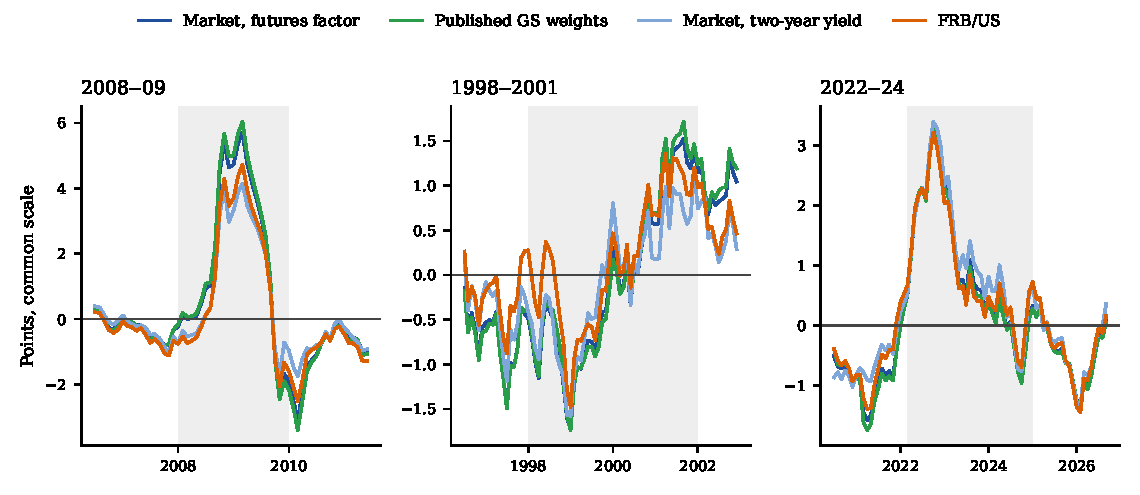
\includegraphics[width=\textwidth]{../replication/report/fig_ep4.pdf}
\caption{Four Readings, Month by Month}
\label{fig:ep4}
\begin{flushleft}\footnotesize\textit{Notes:} Twelve-month change in financial conditions under each portfolio, in points on the common two-year-yield scale, normalized to the futures-factor response. The shaded months are the episodes of Table~\ref{tab:ep4}. Corporate spreads are held fixed.\end{flushleft}
\end{figure}

\textbf{2008--09: the direction is clear, the size is not.} From January 2008 to December 2009 the futures-factor and GS readings average \bl{fw:ep:200809:F} and \bl{fw:ep:200809:G} points of tightening and the two-year-yield and FRB/US readings \bl{fw:ep:200809:Y} and \bl{fw:ep:200809:B}. Equity valuations fell by about half, and the futures-factor and GS portfolios give equities the most weight relative to the dollar and the 10-year yield, so the collapse weighs more in their readings. The four readings are furthest apart in 2009 and 2008, with mean ranges of \bl{fw:topyear:1:range} and \bl{fw:topyear:2:range} points. A policymaker could describe the direction with confidence; the choice of weights changed the estimated tightening by more than half a point. These are readings of three asset prices. Corporate spreads would add to every reading in 2008, by an amount that depends on the spread weight each calibration assigns.

\textbf{1998--2001.} The four readings average \bl{fw:ep:19982001:F} (futures factor), \bl{fw:ep:19982001:G} (GS), \bl{fw:ep:19982001:Y} (two-year yield) and \bl{fw:ep:19982001:B} (FRB/US): three slightly easing and FRB/US slightly tightening, with materially opposing readings in \bl{fw:ep:19982001:opp} months. For the pair of the futures-factor market index and FRB/US, averaged over the episode, the market-implied reading of the 12-month changes was slightly easing, at \bl{ce:1998:dm} points (interval \bl{ce:1998:dm:lo} to \bl{ce:1998:dm:hi}), and the spending-equivalent reading was slightly tightening, at \bl{ce:1998:fr} (\bl{ce:1998:fr:lo} to \bl{ce:1998:fr:hi}). The difference of \bl{ce:1998:D} (\bl{ce:1998:D:lo} to \bl{ce:1998:D:hi}) is a point estimate; its interval includes zero, and so do the intervals for the separate contributions of the dollar (\bl{ce:1998:cusd:lo} to \bl{ce:1998:cusd:hi}) and of equities (\bl{ce:1998:ceq:lo} to \bl{ce:1998:ceq:hi}). The signs differ in the averages and in \bl{ce:1998:opp} of the \bl{ce:1998:nmo} months, and the monthly paths show what the average conceals (Figure~\ref{fig:paths}). The difference was largest in the 12-month changes ending in the first half of 1998, at \bl{mo:19982001:maxgap} points in January 1998, because those changes include the dollar's appreciation and the rise in valuations of 1997, and the model gives the dollar more weight and equities less. It shrank through 1999 and 2000 and turned negative in the second half of 2001 as valuations fell. The disagreement was therefore mostly about size and not direction: the signs differ in only \bl{ce:1998:opp} of \bl{ce:1998:nmo} months, but the readings differ by at least a quarter point in \bl{ce:1998:big}. The dollar appreciated by \bl{ce:1998:xusd} log points a year on average, which adds \bl{ce:1998:cusd} to $D$; equity valuations rose by \bl{ce:1998:xeq} log points a year, which adds \bl{ce:1998:ceq}. Unemployment rose by \bl{ce:1998:real} points over the following year, against forecasts of \bl{ce:1998:fcm} from the market-implied reading and \bl{ce:1998:fcf} from the spending-equivalent reading.


\textbf{2022--24.} Every calibration shows a large tightening: the four readings average \bl{fw:ep:202224:F}, \bl{fw:ep:202224:G}, \bl{fw:ep:202224:Y} and \bl{fw:ep:202224:B}, and no month has materially opposing readings. For the futures-factor pair, the two readings of the 12-month change averaged \bl{ce:2022:dm} points (interval \bl{ce:2022:dm:lo} to \bl{ce:2022:dm:hi}) and \bl{ce:2022:fr} (\bl{ce:2022:fr:lo} to \bl{ce:2022:fr:hi}). Both movements tightened conditions. Equity valuations fell by \bl{abs:ce:2022:xeq} log points a year, and the dollar appreciated by \bl{ce:2022:xusd}. Because the model gives equities less weight than the event study, the fall in equities makes the spending-equivalent reading less tight than the market-implied one, and contributes \bl{ce:2022:ceq} to $D$. Because the model gives the dollar more weight, the appreciation makes the spending-equivalent reading tighter, and contributes \bl{ce:2022:cusd}. The two contributions to the disagreement cancel, so that $D$ averages \bl{ce:2022:D} (\bl{ce:2022:D:lo} to \bl{ce:2022:D:hi}), although each asset tightened conditions. The monthly paths show that the cancellation is not exact at every date: $D$ ranged from about $-0.3$ to $+0.5$ within the episode, and it exceeded 0.25 in absolute value in \bl{ce:2022:big} of \bl{ce:2022:nmo} months. The baseline cancellation is specific to that definition of policy news: with the two-year yield as the signal, $D$ is \bl{sg:two:22D} and the market-implied reading is higher, and without the lower-bound years $D$ is \bl{sg:nlb:22D} (Section~\ref{sec:signal}). A policymaker would have described a sizable tightening under every one of them. The full indexes differ in average level by \bl{br:ep2022:gap} points (interval \bl{br:ep2022:lo} to \bl{br:ep2022:hi}), with the equity weights (\bl{br:ep2022:eq}) and the dollar (\bl{br:ep2022:usd}) both contributing, and that difference does not affect the readings of the year's tightening. Unemployment rose by \bl{ce:2022:real} points over the following year, against forecasts of \bl{ce:2022:fcm} from the market-implied reading and \bl{ce:2022:fcf} from the spending-equivalent reading. Both weightings overpredicted the rise, so the weights do not explain the miss.

\begin{figure}[tbp]
\centering
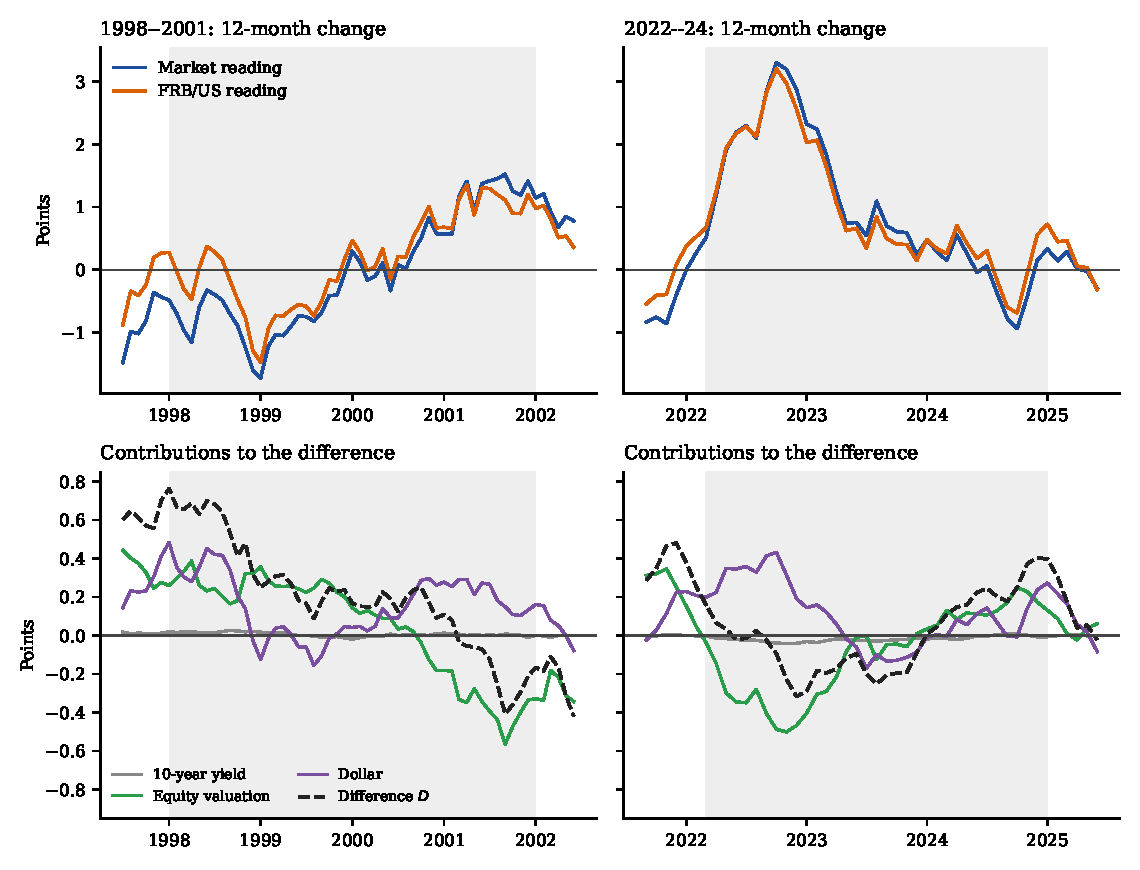
\includegraphics[width=\textwidth]{../replication/report/fig_paths.pdf}
\caption{Month by Month: Readings and the Sources of Their Difference}
\label{fig:paths}
\begin{flushleft}\footnotesize\textit{Notes:} Top: 12-month change of the market-implied and spending-equivalent readings on the same three assets relative to $r^*$. Bottom: each asset's contribution to $D$, the weight difference times its 12-month change, and $D$ itself (dashed). The shaded area is the episode.\end{flushleft}
\end{figure}

\subsection{The Full History}\label{sec:fullhist}
A policymaker reading financial conditions wants to know two things: whether conditions tightened or eased, and by how much. Table~\ref{tab:four} answers both across the four calibrations. All four readings of the 12-month change have the same sign in \bl{fw:all:same:sign} percent of the \bl{fw:nmonths} months (90 percent interval \bl{fw:all:same:sign:lo} to \bl{fw:all:same:sign:hi}). At least two give materially opposing readings, one at least 25 basis points above zero and one at least 25 basis points below, in \bl{fw:any:opposing:t25:n} months (\bl{fw:any:opposing:t25} percent; \bl{fw:any:opposing:t25:lo} to \bl{fw:any:opposing:t25:hi}). With a threshold of 10 basis points the share rises to \bl{fw:any:opposing:t10} percent. Both thresholds belong in view, because what counts as a meaningful disagreement is the policymaker's choice. The size of the change is less robust. The four-reading range, the largest reading less the smallest, is at least 25 basis points in \bl{fw:range:ge:t25} percent of months. That figure answers the question of a policymaker choosing among four calibrations; for one fixed pair, the futures-factor market index and FRB/US, the readings differ by at least 25 basis points in \bl{mo:all:25:big:gap} percent of months (\bl{mo:all:25:big:gap:lo} to \bl{mo:all:25:big:gap:hi}; Table~\ref{tab:months} in the appendix). The intervals are conditional on the observed history and on the fixed FRB/US and GS weights. The rarity of materially opposing readings is the more informative result; how often magnitudes differ is estimated much less precisely.

\begin{table}[tbp]\centering
\caption{How Often the Four Readings Give Different Judgments}\label{tab:four}
\resizebox{\ifdim\width>\textwidth\textwidth\else\width\fi}{!}{%
\begin{tabular}{lrrr}
\toprule
 & Percent of months & 90\% interval & Months \\
\midrule
All four readings have the same sign & 81.6 & [70.2, 82.9] & 301 \\
At least two materially opposing readings, $t$ = 10 bp & 10.3 & [8.4, 19.8] & 38 \\
At least two materially opposing readings, $t$ = 25 bp & 2.2 & [1.6, 8.1] & 8 \\
Four-reading range at least 10 bp & 92.4 & [87.5, 97.6] & 341 \\
Four-reading range at least 25 bp & 70.5 & [58.5, 88.9] & 260 \\
Market (futures factor) and FRB/US materially opposing, $t$ = 25 bp & 2.2 & [0.0, 5.4] & 8 \\
\bottomrule
\end{tabular}}
\begin{flushleft}\footnotesize\textit{Notes:} Monthly 12-month changes in the three assets relative to $r^*$, January 1996 to September 2026 (369 months, overlapping), read with the four portfolios on the common two-year-yield scale. Materially opposing: at least one reading at least $t$ above zero and at least one at least $t$ below zero. Four-reading range: the largest less the smallest of the four readings. Intervals: 5th and 95th percentiles over 5,000 bootstrap draws of the announcements (market weights and the common response vector redrawn; FRB/US and GS weights fixed), conditional on the observed history.\end{flushleft}
\end{table}


\textbf{The exceptions.} Table~\ref{tab:opp} lists the \bl{fw:any:opposing:t25:n} months of materially opposing readings. They fall in four periods, 1997--98, 2003, 2008 and 2015, and show two patterns. In \bl{fw:opp25:Balone} months, in late 1997, the first half of 1998 and early 2015, FRB/US alone reads a tightening of at least 25 basis points while the others read an easing. In each of those months the dollar had risen by more than 10 percent over the year, valuations had also risen by more than 10 percent and the 10-year yield had fallen. FRB/US gives the dollar the largest weight relative to equities, so the appreciation dominates its reading; the others give more weight to the rise in valuations and the fall in yields. In the other \bl{fw:opp25:FGtight} months, May 2003 and June 2008, the futures-factor and GS readings are tight while FRB/US is easy. Valuations had fallen by more than 20 percent over the year and the dollar had depreciated, and those two portfolios weight equities most heavily relative to the dollar.

\begin{table}[tbp]\centering\small
\caption{The Months of Materially Opposing Readings}\label{tab:opp}
\resizebox{\ifdim\width>\textwidth\textwidth\else\width\fi}{!}{%
\begin{tabular}{lrrrrll}
\toprule
Month & Market, futures factor & Published GS weights & Market, two-year yield & FRB/US & Tighter (at least 25 bp) & Easier (at least 25 bp) \\
\midrule
Dec 1997 & $-$0.43 & $-$0.40 & $-$0.24 & 0.27 & FRB/US & Market, futures factor, Published GS weights \\
Jan 1998 & $-$0.49 & $-$0.41 & $-$0.42 & 0.28 & FRB/US & Market, futures factor, Market, two-year yield, Published GS weights \\
Jun 1998 & $-$0.33 & $-$0.27 & $-$0.23 & 0.37 & FRB/US & Market, futures factor, Published GS weights \\
Jul 1998 & $-$0.39 & $-$0.35 & $-$0.26 & 0.29 & FRB/US & Market, futures factor, Market, two-year yield, Published GS weights \\
May 2003 & 0.41 & 0.53 & $-$0.28 & $-$0.30 & Market, futures factor, Published GS weights & Market, two-year yield, FRB/US \\
Jun 2008 & 0.46 & 0.56 & $-$0.18 & $-$0.26 & Market, futures factor, Published GS weights & FRB/US \\
Mar 2015 & $-$0.37 & $-$0.30 & $-$0.37 & 0.26 & FRB/US & Market, futures factor, Market, two-year yield, Published GS weights \\
Apr 2015 & $-$0.37 & $-$0.30 & $-$0.35 & 0.25 & FRB/US & Market, futures factor, Market, two-year yield, Published GS weights \\
\bottomrule
\end{tabular}}
\begin{flushleft}\footnotesize\textit{Notes:} Twelve-month change in financial conditions under each portfolio, on the common two-year-yield scale (points), in the months in which at least one reading is at least 0.25 above zero and at least one at least 0.25 below zero.\end{flushleft}
\end{table}

\FloatBarrier

% ============================================================
\section{What Can Subsequent Activity Establish?}\label{sec:outlook}
\subsection{The Test}\label{sec:onetest}
Consider two years in which the market index tightened by the same amount. If the dollar accounted for more of the tightening in one year, did activity subsequently weaken more? If the market-implied reading is a sufficient summary of the asset prices, the answer is no. If the spending-equivalent reading is, the answer is yes, by the amount that the model's weights imply. I regress the 12-month-ahead change in the unemployment gap on own lags and
\begin{equation}\label{eq:test}
y_{t+12}-y_t=\cdots+\beta M_t+\gamma D_t ,
\end{equation}
where $M$ is the 12-month change in the market index (relative to $r^*$) and $D$ the 12-month change of the normalized FRB/US-minus-market difference on the same changes. If the market-implied reading is sufficient, $\gamma=0$. If the spending-equivalent reading $M+D$ is sufficient, $\gamma=\beta$. I read the two restrictions as tests of incremental predictive sufficiency in the span of the two portfolios, conditional on the controls. Three assets span a larger space, and an unrestricted regression on the three assets is a different test. Failure to separate the portfolios for aggregate unemployment or GDP is consistent with low power and with forward-looking asset prices, and it cannot validate either structural weight. That wording matters for unemployment, since the FRB/US weights are constructed from effects on GDP; four-quarter GDP growth is the model-facing check. Table~\ref{tab:comp} reports both restrictions with the joint covariance of the estimates. The test compares two of the four calibrations, the futures-factor market reading and the FRB/US reading.

\subsection{The Answer}\label{sec:answer}
On 1976--2026 the coefficient on the index change is \bl{rs:du:main:beta} and on composition \bl{rs:du:main:gamma} (\bl{rs:du:main:gamma:lo} to \bl{rs:du:main:gamma:hi}); the difference $\gamma-\beta$ is \bl{rs:du:main:gmb} (\bl{rs:du:main:gmb:lo} to \bl{rs:du:main:gmb:hi}). Neither restriction is rejected. Moving $D$ from its 5th to its 95th percentile at the same index change shifts the year-ahead outlook by \bl{cm:du:main:eff} percentage point, with an interval from \bl{cm:du:main:efflo} to \bl{cm:du:main:effhi}, so the sample cannot establish an outlook difference of either sign. On 1996--2026 the coefficient on the index change is \bl{rs:du:1996p:beta} (\bl{rs:du:1996p:beta:lo} to \bl{rs:du:1996p:beta:hi}) and on composition \bl{rs:du:1996p:gamma} (\bl{rs:du:1996p:gamma:lo} to \bl{rs:du:1996p:gamma:hi}) and the model's restriction is rejected ($\gamma-\beta=$ \bl{rs:du:1996p:gmb}, \bl{rs:du:1996p:gmb:lo} to \bl{rs:du:1996p:gmb:hi}); excluding 2008--15 the coefficient on composition is \bl{rs:du:ex200815:gamma} and $\gamma-\beta$ is \bl{rs:du:ex200815:gmb}, close to the model's restriction. The sign changes across samples. For GDP growth neither restriction is rejected, and adding $D$ does not significantly improve out-of-sample forecasts (Clark--West \bl{cm:addD:cw}).

\begin{table}[tp]\centering\small
\caption{Does the Composition of a Tightening Matter for the Outlook?}\label{tab:comp}
\resizebox{\ifdim\width>\textwidth\textwidth\else\width\fi}{!}{%
\begin{tabular}{lrrrr}
\toprule
 & $n$ & Index change & Composition $D$ [90\%] & Outlook difference, 5th to 95th percentile [90\%] \\
\midrule
Unemployment gap, 12 months: 1976--2026 & 556 & 0.19 & $-$0.27 [$-$0.96, 0.42] & $-$0.30 [$-$1.06, 0.47] \\
Unemployment gap, 12 months: 1996--2026 & 318 & 0.01 & $-$1.18 [$-$2.51, 0.14] & $-$1.10 [$-$2.33, 0.13] \\
Unemployment gap, 12 months: Excluding 2008--15 & 436 & 0.29 & 0.32 [$-$0.13, 0.77] & 0.36 [$-$0.15, 0.86] \\
Real GDP growth, four quarters: 1976--2026 & 186 & $-$0.16 & 0.89 [$-$0.77, 2.55] & 0.97 [$-$0.84, 2.79] \\
Real GDP growth, four quarters: 1996--2026 & 106 & 0.31 & 1.82 [$-$0.77, 4.40] & 1.60 [$-$0.68, 3.89] \\
Real GDP growth, four quarters: Excluding 2008--15 & 146 & $-$0.33 & 0.27 [$-$1.20, 1.75] & 0.31 [$-$1.37, 2.00] \\
\bottomrule
\end{tabular}}
\begin{flushleft}\footnotesize\textit{Notes:} Local projections of the 12-month-ahead change in the unemployment gap (four-quarter-ahead GDP growth) on own lags, the 12-month change of the market index relative to $r^*$ and the 12-month change of the normalized FRB/US-minus-market difference $D$ computed on the same changes (HAC standard errors, 18 lags; the intervals from block bootstrap are similar). Outlook difference: the coefficient on $D$ times the difference between the 5th and 95th percentiles of $D$ at a given index change, in percentage points of the unemployment gap (percent for GDP). If the FRB/US weights were right, the coefficient on $D$ would equal the coefficient on the index change.\end{flushleft}
\end{table}


What can a policymaker take from this? The two readings can be used interchangeably when markets move as they do around policy news, and the data cannot say which to prefer when they do not. A reading from either index should be accompanied by the question of what moved: the dollar, valuations, or yields. The answer indicates whether the two readings are likely to part.


\FloatBarrier

% ============================================================
\section{How Stable Are the Weights, and What Are the Limits?}\label{sec:limitsmain}
\subsection{Weights That Move}\label{sec:drift}
The weights define the unit, so I hold them fixed and show how they would drift. Re-estimating on an expanding window of announcements from 2006 keeps the 10-year and dollar weights inside the 90 percent band of the full-sample estimate at every date after 2010; the equity weight is outside the full-sample 90 percent bootstrap interval in \bl{exp:n} monthly estimates between \bl{exp:first} and \bl{exp:last}, by at most \bl{exp:post2010:min:eq} against a band edge of \bl{base:lo:eq} (Figure~\ref{fig:weightpath}). The overlapping monthly estimates are not \bl{exp:n} independent tests of instability. A 20-year rolling window fails after 2021, because it drops the announcements of 1996--2005. The 10-year weight is imprecise throughout. Apart from the equity weight in these years, the weights stay within their sampling error.

\begin{figure}[tbp]
\centering
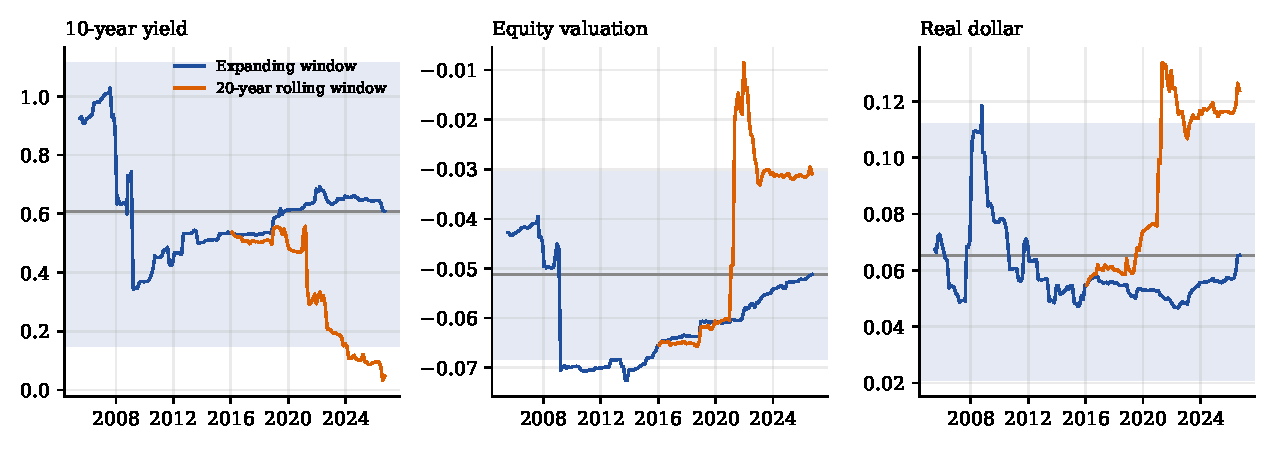
\includegraphics[width=\textwidth]{../replication/report/fig_weight_path.pdf}
\caption{The Weights on an Expanding and a Rolling Window}
\label{fig:weightpath}
\begin{flushleft}\footnotesize\textit{Notes:} Weights of the market index re-estimated on announcements to each date (expanding window, from the 80th announcement) and on the latest 20 years (rolling). Shaded: 90 percent bootstrap interval of the full-sample weights; the horizontal line is the full-sample weight.\end{flushleft}
\end{figure}


The other policy-news series and event samples are in Appendix~\ref{sec:robother}.

\subsection{Limits of the Design}\label{sec:limits}
The weights come from announcements since 1996 and are applied from 1973; they assume that the responses reflect policy rather than information effects \citep{nakamura2018}, and if policy came to target financial conditions the responses could change, the Lucas-critique concern that \citet{hatzius2010} raise for all indexes. The FRB/US weights come from one model, at one horizon and in one experiment, and are held fixed in the intervals. The daily comparison of Section~\ref{sec:size} uses nominal assets, with the nominal broad dollar for the real dollar, no adjustment for $\rs$ and weights fitted on the same announcements; the intraday comparison holds each event out. The sample has five recessions, two of them out of sample, and the 12-month outcomes overlap, so the counts of tests are descriptive and not adjusted for their number. The neutral rate is not neutral to outcomes, because the Laubach--Williams model uses output, inflation and unemployment.

\FloatBarrier

% ============================================================
\section{Conclusion}\label{sec:discussion}
The paper asks how many points of monetary policy a movement in financial conditions is worth. An event study says how large a conventional policy surprise the movement resembles, and a spending calibration says how large a policy-rate change would have a comparable effect on GDP. The two questions are different. Knowing which one an index answers, however, tells a reader surprisingly little about which other index it will resemble. On the movements of Figure~\ref{fig:four} the futures-factor market index and the published Goldman Sachs weights give nearly the same relative readings, and the two-year-yield market index and FRB/US both give the appreciation more than twice the reading of the equity decline.

Across four calibrations put on one scale, financial conditions usually give the same directional signal. Over 1996--2026 all four readings of the annual change have the same sign in \bl{fw:all:same:sign} percent of months, and materially opposing readings occur in \bl{fw:any:opposing:t25:n} of \bl{fw:nmonths} months at a threshold of 25 basis points. The size of the tightening is more sensitive. Switching between two implementations of the same method can change the reading as much as switching from market responses to spending effects, and the two closest readings in the sample come from different methods, on the paper's series and on series closer to the GS inputs. In 2008--09 every calibration showed a large tightening and the size differed by more than half a point; in 2022--24 the weights differed and the readings nearly converged. The weights differ for reasons the paper can trace: the measure of policy news on the market side, and the trade channel of the dollar in FRB/US. Why the published Goldman Sachs weights match the futures-factor market weights is open.

GDP growth provides little evidence for choosing between the futures-based market reading and the FRB/US reading, and the unemployment comparison is sensitive to the sample. The FRB/US weights come from one model and one experiment and the published weights are applied to series they were not built on, so the four portfolios are a defined set of U.S.\ calibrations and not the population of indexes. For a policymaker, the practical reading is that the direction of a change in financial conditions is a robust signal across reasonable ways of translating it into policy-rate points, and its size is not. A reading of a quarter point of equivalent tightening should come with the calibration that produced it and with what moved: the dollar, valuations or yields.
\FloatBarrier
